\chapter{Results \& Discussion}
%\textbf{Should include a reiteration of the experiments, and their outcome.  Together with a description (discussion).  Preamble should include a reminder of the aims and objectives together with a list of experiments to achieve these.  Should include many charts and other visualization with appropriate descriptions}.  
Recall that we split the practical work in two categories.  In this first instance, we tested the reviewed projection learning algorithms on a common dataset and evaluation metrics as well as multiple embedding spaces.  We aimed for more statistical rigour than was presented in the original papers.  In the second set of experiments, we focused on CRIM, an easy-to-train algorithm which performed well in our experiments and was the best submission in the Semeval-2018, Task 9 challenge.  We explored it in some detail within the context of the shared task \citep{camacho2018semeval}.  

\section{Dataset Statistics} \label{dataset_stats}
To fully appreciate the results, we need to foster familiarity with the datasets used to train and evaluate our models.  In this section, we outline the main datasets used in our experiments, in terms of their descriptive statistics.  

\subsection{Combined Dataset}
We use a standard, highly curated dataset - actually an amalgam of four datasets - to run a comparative study of each reviewed projection learning model.   We refer to this dataset throughout this dissertation as the \textit{Combined Dataset}.  
\begin{table*}\centering
\begin{tabular}{@{}llr@{}}\toprule
\multicolumn{3}{c}{\textbf{Combined Dataset}} \\ \midrule
\multicolumn{2}{c}{Total Tuples} & 7,397\\
\multicolumn{2}{c}{Unique Queries} & 2,259\\ \midrule
\multirow{3}{*}{Hypernyms} & Unique & 1,453\\
& Max & 17\\
& Mean & 3.274\\
Synonyms & Query terms, $\vert syn \vert > 0$ & 877\\
\bottomrule
\end{tabular}
\caption{Combined Dataset statistics.}\label{tab:combined_dataset_stat}
\end{table*}

Table~\ref{tab:combined_dataset_stat} reflects the Combined Dataset's key statistics.  It contains a total of 7,397 tuples which we will split in five folds, dedicating 5,918 tuples in each fold for training the models and 1,479 for validation\footnote{The exact numbers may vary depending on the embeddings used; in this case we assume word2vec.}.  There are 2,259 distinct query (or hyponym) terms which are mapped to 1,453 distinct hypernyms.  74\% of the query terms are associated with one to four hypernyms, where a hyponym is linked to a mean 3.3 hypernyms.  Less than 50 hyponyms are mapped to 10 or more hypernyms each.  Example terms include wearable items such as \textit{cloak} (11), \textit{glove} (12); and animals such as \textit{fox} (10), \textit{cow} (14).  

The words in the Combined Dataset largely pertain to the biology domain: 2,295 tuples (31\% of the total dataset) feature one of 8 hypernyms (0.55\% of all distinct hypernyms in the set) which categorise some aspect of the natural world.  The top three most frequent hypernyms are \textit{animal}, \textit{plant} and \textit{chordate} which occupy the hypernym slot of 497, 440 and 363 word-pairs respectively.  The Combined Dataset also features a set of synonyms which we use to adjust our models' loss via neighbour regularisation.  There is at least one synonym for 39\% of the hyponyms.

\subsection{Shared Task Dataset}
\begin{table*}\centering
\begin{tabular}{@{}llrcrcr@{}}\toprule
\multicolumn{7}{c}{\textbf{Semeval-2018, Task 9 Dataset}} \\ \midrule
& & \textbf{Concept} & \phantom{a} & \textbf{Entity} & \phantom{a} & \textbf{Both} \\
\cmidrule{3-3} \cmidrule{5-5} \cmidrule{7-7}
\multirow{3}{*}{Training} & \textit{\# Tuples} & 7,184 && 4,595 && 11,779 \\
& \textit{Uniq. Hypo.} & 979 && 521 && 1,500\\
& \textit{Uniq. Hyper.} & 3,476 && 1,426 && 4,233\\ 
\cmidrule{2-7}
\multirow{3}{*}{Test} & \textit{\# Tuples} & 4,936 && 2,112 && 7,048 \\
& \textit{Uniq. Hypo.} & 1,057 && 443 && 1,500\\
& \textit{Uniq. Hyper.} & 2,575 && 812 && 3,076\\
\cmidrule{2-7}
\multirow{3}{*}{\textbf{Total}} & \textit{\# Tuples} & \textbf{12,120} && \textbf{6,707} && \textbf{18,827} \\
& \textit{Uniq. Hypo.} & 2,036 && 964 && 3,000\\
& \textit{Uniq. Hyper.} & 4,703 && 1,722 && 5,556\\
\bottomrule
\end{tabular}
\caption{Semeval-2018 Task 9, English general-purpose dataset statistics.}\label{tab:semeval_dataset_stat}
\end{table*}

For this dissertation we focused on the general-purpose English dataset shipped with the Shared Task.  The organisers split the dataset into training, test and validation subsets and, since we will be comparing our results to the other participants' work, we use the data as they were delivered.  The dataset's descriptive statistics can be viewed in Table~\ref{tab:semeval_dataset_stat}, excluding the validation split which only consists of 200 tuples.

It is immediately evident that the Shared Task Dataset is larger, and more diverse than the Combined Dataset.  In total, the dataset features 18,827 tuples - 2.54 times the size of the Combined Dataset - where each hyponym is associated with an average of 6.3 hypernyms.  The query terms are divided evenly between the training and test datasets.  Roughly 30\% of the terms are entities (proper nouns) and, therefore, \textit{instances} rather than \textit{subclasses} of their designated hypernyms.  We can see that the unique hypernym counts are not perfectly additive across the rows and columns of the table.  This is because some hypernyms are relatively more frequent than other and linked with terms in both the training and test sets.  However, this dataset is less bound to a particular domain than the Combined Dataset.  Indeed, \textit{person} is the highest frequency hypernym but is only mapped to 612 tuples or 3.25\% of the entire dataset.
\begin{figure}[ht!] 
  \centering
  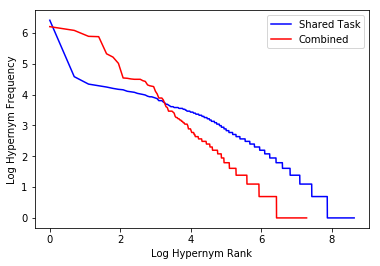
\includegraphics[width=0.5\linewidth]{images/both_hyper_freq_zipf.png}
  \caption{Log-log plot of hypernym rank against frequency, Combined and Shared Task datasets.}
  \label{fig:dataset_hypernym_freq}
\end{figure}
We illustrated the distribution of hypernyms in the datasets by plotting the log hypernym rank against the log frequency in Figure~\ref{fig:dataset_hypernym_freq}.  Hypernym frequency in the Combined Dataset follows a Zipf-like distribution, although clearly, the highest ranking hypernyms have similar frequencies.  In the Shared Task case,  the plot is generally shallower and less akin to a Zipf distribution.  The frequency of the top ranked hypernyms initially falls sharply and then decreases slowly from the 7$^{th}$ ranked hypernym onward.
\begin{figure}[ht!] 
  \centering
  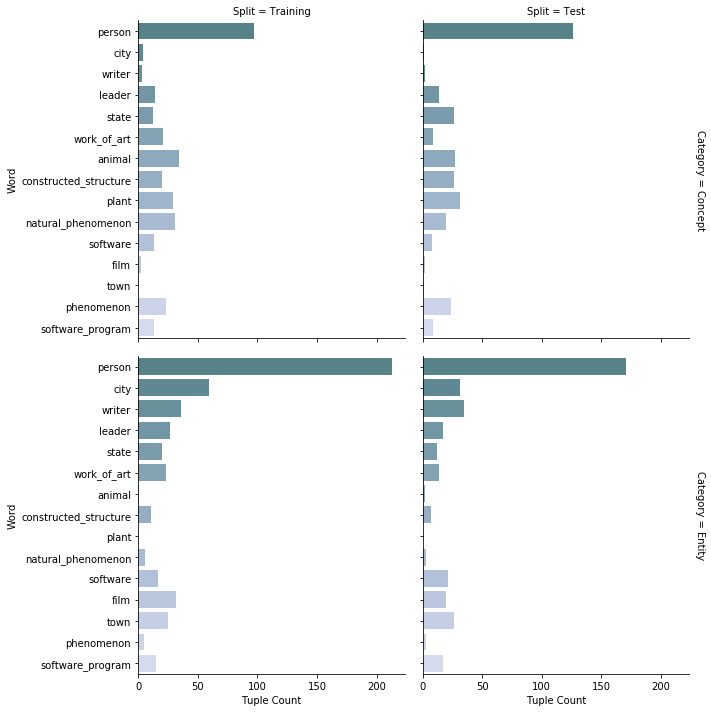
\includegraphics[width=0.75\linewidth]{images/shared_task_MFH.png}
  \caption{Distribution of the most frequent hypernyms in the Shared Task dataset.}
  \label{fig:shared_task_mfh}
\end{figure}
The Shared Task dataset is split in four partitions between training/test splits and concept/entity hyponym word types.  We plotted the distribution of the 15 most frequent hypernyms in the overall dataset with respect to each partition in Figure~\ref{fig:shared_task_mfh}.  The word \textit{person} features conspicuously as a frequent hypernym in every data partition with a considerable margin over \textit{city}, the second most frequent hypernym overall.  This is consistent with Figure~\ref{fig:dataset_hypernym_freq}.

The distribution of training and test samples seems to be fairly uniform, at least in terms of the 15 most-common hypernyms.  In general, entities are more likely to be defined by frequent hypernyms.  This is understandable since named entity labels are narrower in scope than concepts which encompass all common nouns.  The popularity of hypernyms like \textit{city}, \textit{state}, and \textit{leader}, might be an  indication that \textit{UMBC} corpus leans towards geo-political content, but this is tenuous evidence at best.  Lastly, we observe that the natural world is not as over-represented as it was in the Combined Dataset, although \textit{animal} and \textit{plant} are still among the 15 most frequent hypernyms in the Shared Task dataset too.

\section{Hard-Clustering and Regularisation}
\subsection{Objectives}
\citeauthor{ustalov2017negative} proposed a set of regularistion terms, minimised together with the \ac{MSE} objective function, designed to uphold the asymmetric nature of the hypernymy relation and discourage the model from projecting a query term close to its synonyms \citep{ustalov2017negative}.  We felt that the proposals were interesting but that the study's evidence of their efficacy was statistically weak.  Meanwhile, the chosen evaluation metrics - although sound - did not make it possible to compare the models with their projection learning peers \citep{yamane2016distributional, bernier2018crim}.  

We aimed to peruse of a standard set of metrics and employ a slightly-modified implementation provided by the SemEval-2018, Task 9 organisers \citep{camacho2018semeval}.  Moreover, we refactored the experimental setup such that we produce a distribution of scores from a cross-validated dataset which allowed us to conduct a \textit{difference of means} hypothesis test.  Finally, we tested several embeddings feature spaces for observable differences in performance.

\subsection{Effect of Training Piecewise Projections}
\begin{figure}[ht!] 
  \centering
  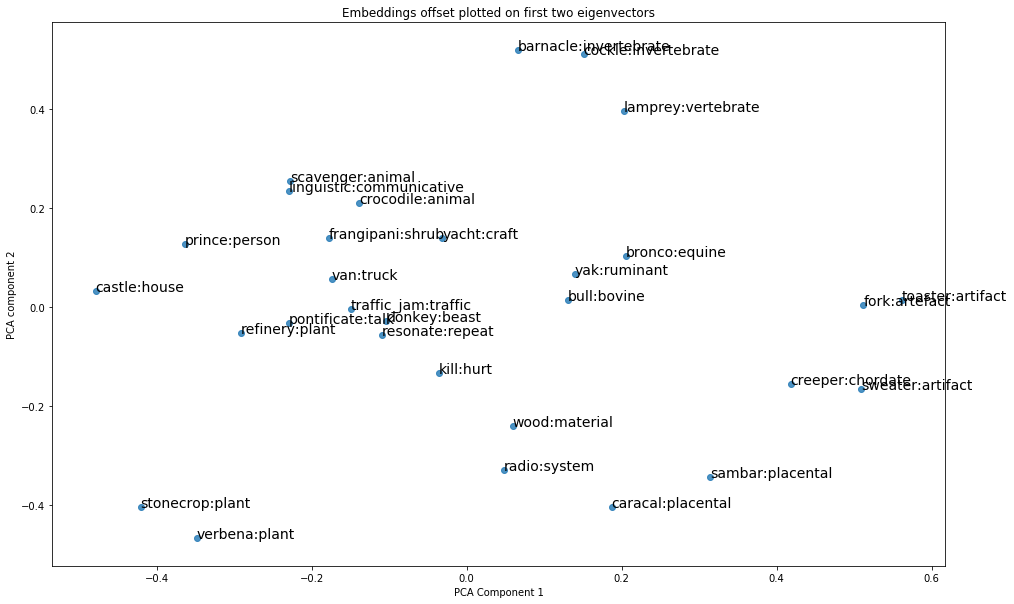
\includegraphics[width=0.75\linewidth]{images/Sample_of_30_vector_offsets_PCA.png}
  \caption{Sample of 30 vector offsets projected on first two PCA components.}
  \label{fig:cluster_30_samp_pca}
\end{figure}
We evaluated single-cluster models that learned one transformation matrix for all the samples in the training dataset and multi-cluster models that first partition the word-pairs exclusively into a declared number of clusters.  We plotted 30 random vector offset samples projected on the first two eigenvectors of the word2vec embeddings space reduced by \ac{PCA}.  Despite that the PCA model only explains 15\% of the variance of the 30 samples, distinct clusters can be observed in Figure~\ref{fig:cluster_30_samp_pca}.  Plant vector (offsets) are occupying a cluster towards the bottom-left of the figure; \textit{equine}, \textit{ruminant} and \textit{bovine} vectors are clumped in a cluster at the centre of the plot whereas \textit{fork} and \textit{toaster} are grouped due to them being \textit{artefacts}.

\begin{figure}[ht!] 
  \centering
  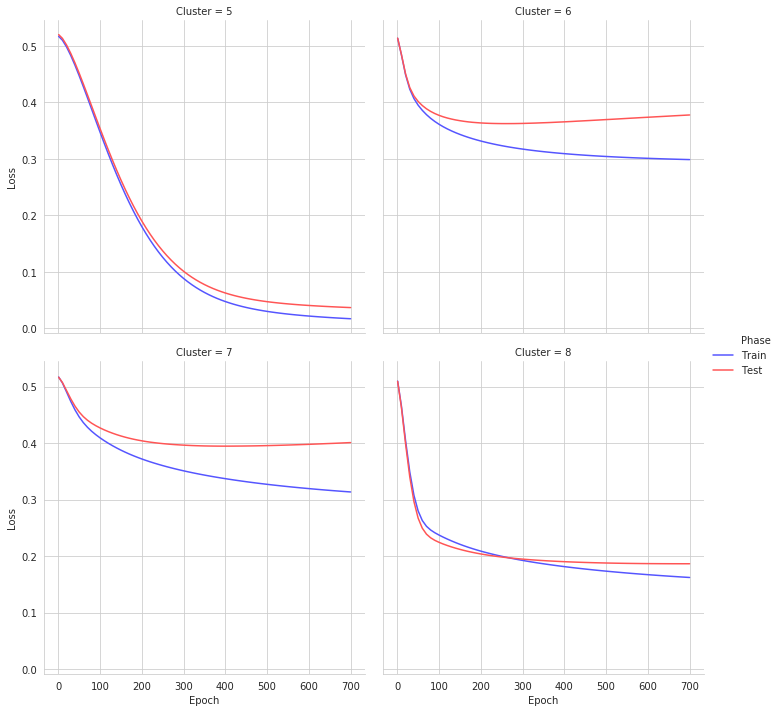
\includegraphics[width=0.75\linewidth]{images/Train_losses_4_clusters_baseline_w2v.png}
  \caption{Train and validation loss on 4 data clusters (Baseline, word2vec).}
  \label{fig:train_test_loss_w2v}
\end{figure}

The training experience on the clusters differed.  We recorded the training and test loss returned when training a 10-cluster, baseline (i.e. no regularisation) model on an arbitrary training fold. This is the \citep{Fu2014} baseline as implemented in \citep{ustalov2017negative}.  We reproduced train and test losses for four clusters, chosen because of their idiosyncratic performance, in Figure~\ref{fig:train_test_loss_w2v}.

In some cases, such as \textit{cluster 5} (top-left panel), the cluster contained word-pairs featuring a distinctive linear relation between hyponym and hypernym vectors, a fact which was captured by the model.  The test loss mirrors the training loss almost perfectly which suggests that the members of the 5$^{th}$ test cluster belong to the same semantic family of the word-pairs in the training cluster.  The 6$^{th}$ and 7$^{th}$ cluster do not fare as well: over-fit is manifested at the 150-200 epoch mark and the end-of-training loss is markedly higher than what was observed in the 5$^{th}$ cluster.  A balanced performance was delivered by the 8$^{th}$ cluster: no conspicuous over-fit and a reasonable end-of-training loss.

\subsection{Baseline against Regularised Model Results}
\begin{figure}[ht!] 
  \centering
  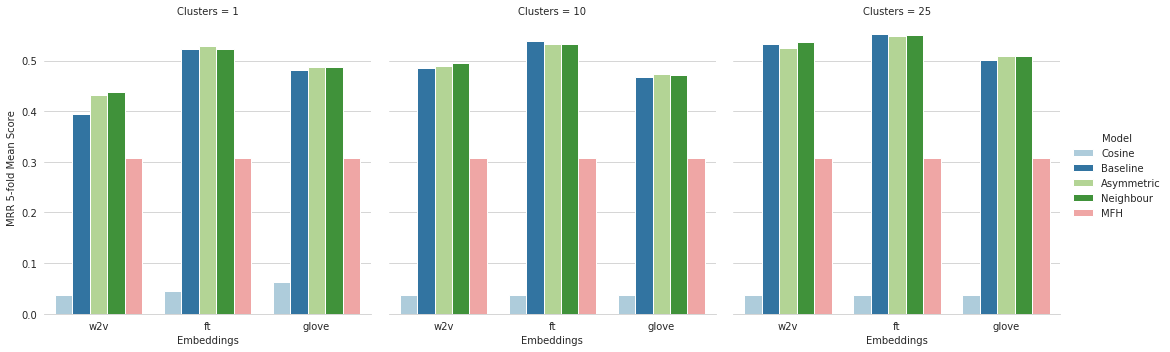
\includegraphics[width=1.\linewidth]{images/MRR_5-fold_results_models_baselines_embeddings.png}
  \caption{MRR cross-validated results, by cluster size, baselines, models and embeddings.}
  \label{fig:MRR_models_baselines}
\end{figure}

\begin{figure}[ht!] 
  \centering
  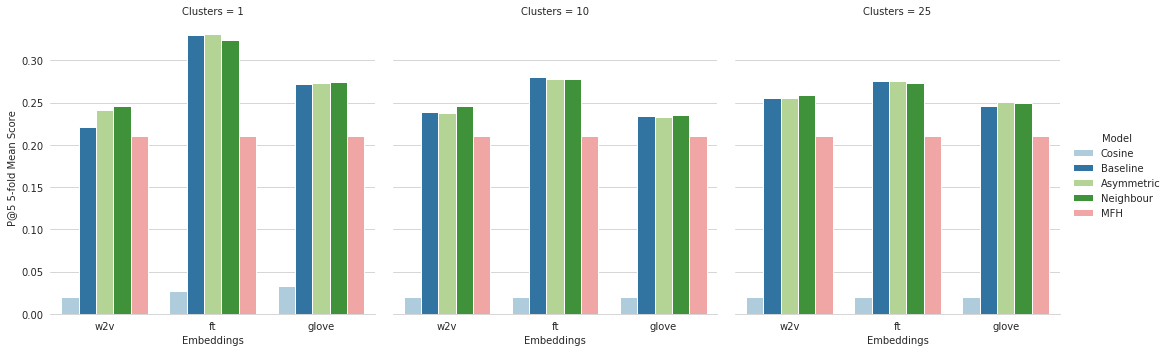
\includegraphics[width=1.\linewidth]{images/PAt5_5-fold_results_models_baselines_embeddings.png}
  \caption{P$@5$ cross-validated results, by cluster size, baselines, models and embeddings.}
  \label{fig:pat5_models_baselines}
\end{figure}

We measured the models' performance on the basis of 5 metrics: \ac{MRR}, \ac{MAP}, and P$@k$ where $k \in \{1, 5, 10\}$.  We report MRR, MAP results since they were largely found to be uncorrelated according to the Spearman rank-order correlation test. \footnote{The only exceptions were the word2vec MAP, MRR results which were correlated with a score of 0.988 at 99\% confidence.}   We also report P$@5$ results for completeness but omit P$@1$ and P$@10$ due to space considerations.  P$@k$ results are positively correlated with \ac{MAP} according to the Spearman's rank-order correlation.

According to our cross-validated experiments on randomly-split datasets, the regularised models exert only a slight influence on the results, except for those observed on the single cluster model trained on word2vec embeddings features.  MRR scores are plotted in Figure~\ref{fig:MRR_models_baselines}.  MRR rewards models for which the first discovered, correct hypernym per term is ranked highly.  \citeauthor{ustalov2017negative}'s modifications slightly harm the models in the fastText 10 and 25 cluster scenarios.  The most-pronounced effect of regularisation was observed with the single-cluster model trained on word2vec embeddings features.  MRR improved by 9.5\% and 11.2\%  with the asymmetric and neighbour regularisation models respectively.  P$@5$ results are plotted in Figure~\ref{fig:pat5_models_baselines}.  Similar to the MRR results, regularisation has left the largest impact on the single-cluster model trained on word2vec features.
\begin{table*}\centering
\begin{tabular}{@{}lrrcrrcrrcrr@{}}\toprule
& \multirow{2}{*}{MFH} & \multirow{2}{*}{Cos} & \phantom{a} &  \multicolumn{2}{c}{\textit{Baseline}} & \phantom{a} & \multicolumn{2}{c}{\textit{Asymmetric}} & \phantom{a} & \multicolumn{2}{c}{\textit{Neighbour}}\\
\cmidrule{5-6} \cmidrule{8-9} \cmidrule{11-12}
&  &  && $\bar{x}$ & $\pm\sigma_{\bar{x}}$ && $\bar{x}$ & $\pm\sigma_{\bar{x}}$ && $\bar{x}$ & $\pm\sigma_{\bar{x}}$ \\ \midrule
\textbf{word2vec}\\
\textit{1} & 0.204 & 0.019 && 0.227 & 0.016 && 0.249 & 0.010 && 0.253 & 0.011 \\
\textit{10} & 0.204 & 0.019 && 0.254 & 0.011 && 0.253 & 0.020 && 0.261 & 0.011 \\
\textit{25} & 0.204 & 0.019 && 0.275 & 0.008 && 0.273 & 0.016 && 0.278 & 0.011 \\
\cmidrule{2-12}
\textbf{GloVe}\\
\textit{1} & 0.204 & 0.032 && 0.284 & 0.015 && 0.285 & 0.019 && 0.285 & 0.014 \\
\textit{10} & 0.204 & 0.019 && 0.248 & 0.019 && 0.248 & 0.034 && 0.250 & 0.020 \\
\textit{25} & 0.204 & 0.019 && 0.262 & 0.013 && 0.268 & 0.017 && 0.267 & 0.012 \\
\cmidrule{2-12}
\textbf{fastText}\\
\textit{1} & 0.204 & 0.025 && \textbf{0.339} & 0.019 && \textbf{0.341} & 0.014 && \textbf{0.334} & 0.015 \\
\textit{10} & 0.204 & 0.019 && \textbf{0.295} & 0.024 && \textbf{0.291} & 0.010 && \textbf{0.292} & 0.021 \\
\textit{25} & 0.204 & 0.019 && \textbf{0.293} & 0.009 && \textbf{0.293} & 0.020 && \textbf{0.292} & 0.012 \\
\bottomrule
\end{tabular}
\caption{5-fold cross-validated \ac{MAP} results for \ac{MSE} model variants trained on three embeddings spaces.}\label{tab:map_mse}
\end{table*}
Our experiments' \ac{MAP} scores are reproduced in Table~\ref{tab:map_mse}.  In this table we are comparing the performance of the various regularised models against a non-na\"ive baseline, while also showing score variations based on three cluster sizes and embeddings.  For comparison, we also included two na\"ive baselines: MFH and Cosine similarity.  We marked the overall best \ac{MAP} results in bold.  The re-projected neighbour regularised model enjoyed the widest improvement margin, increasing the mean \ac{MAP} by around 11.5\% from 0.227 to 0.253 but this performance was isolated to the single-cluster model.  Improvement was either exceedingly subtle (e.g. GloVe, clusters=10) or altogether absent (e.g. fastText, clusters=1).  We evaluate these results statistically in \cref{Eval_MSE}.

\subsection{Single Cluster against Multi-Cluster Model Results}
Increasing the cluster size seems to have a favourable effect on the word2vec models in most cases, particularly when training a 25-cluster baseline model for which a 21.1\% \ac{MAP} score improvement over the single-cluster variant was registered.  Less pronounced improvements were recorded on the regularised models while a 10-cluster model had a moderate effect on \ac{MAP} where the widest improvement margin (21.1\%) was only noted with the baseline model.  

Increasing cluster size had a detrimental effect on models trained on GloVe embeddings.  Specifically, the \ac{MAP} scores dipped for the baseline and neighbour regularisation models while the asymmetric model fared similarly.  The deterioration was not as conspicuous between the single cluster and 25-cluster models, although the performance of the latter suffered compared to the smaller model.  

Multi-clusters harmed the fastText models even more.  All single-cluster models were better-performing than the 10-cluster and 25-cluster variants, whereby every multi-cluster model suffered an average decrease of 13.4\% of its corresponding single-cluster \ac{MAP} score.  

\subsection{Embeddings Effect} \label{ustalov_embeddings}
We observed the overall best \ac{MAP} result with a single-cluster model trained on fastText embeddings with asymmetric regularisation (0.341).  Moreover, fastText \ac{MAP} results were the best in every other category, suggesting that the feature space exerts a greater influence on the \ac{MSE} models' performance than either cluster size or regularisation.  The hypothesis will be evaluated statistically in \cref{Eval_MSE}.

The mean GloVe embeddings' \ac{MAP} score was only higher than the corresponding word2vec models in the single-cluster experiments.  In the 10 and 25-cluster configurations, GloVe features yielded the worst results.  We shall determine if GloVe was significantly worse when evaluating the results according to the \ac{ANOVA} framework in \cref{Eval_MSE}.

\subsection{Na\"ive Baselines}
We also note from Figures~\ref{fig:MRR_models_baselines},~\ref{fig:pat5_models_baselines} and Table~\ref{tab:map_mse} that all trained models have a considerable edge on the na\"ive baselines.  The \ac{MFH} yields better results than cosine similarity across the base, but is bettered by even the worst-performing trained model in all scenarios.  

%% Results are interpreted in the evaluation.  Significant is only observed in one particular scenario - w2v; single cluster.
\subsection{Lexically-Split Experiment Results}
\begin{figure}[ht!] 
  \centering
  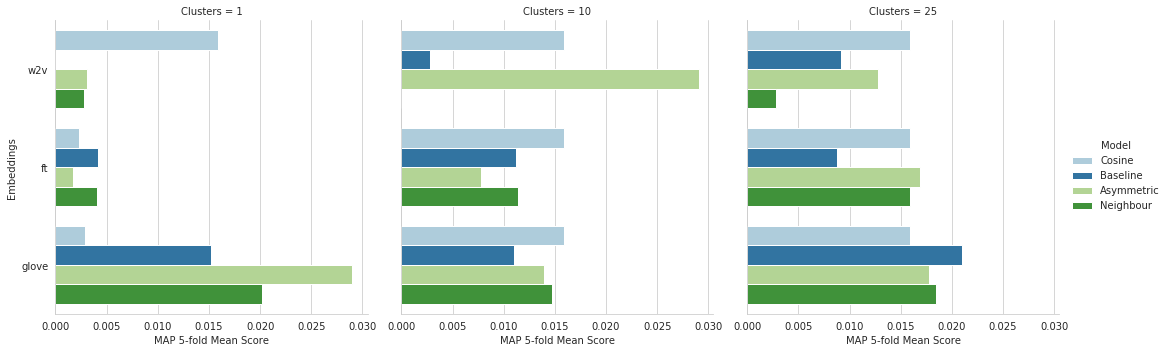
\includegraphics[width=1.\linewidth]{images/MAP_lexical_split_results_models_baseline_embeddings.png}
  \caption{Lexical-split dataset \ac{MAP} results, by model, embeddings.}
  \label{fig:lexsplit_ustalov_map}
\end{figure}
In the lexically-split dataset, we ensured that a word in the hypernym slot of a word-pair either features in training set or the test set but not in both.  The \ac{MAP} results are reproduced in Figure~\ref{fig:lexsplit_ustalov_map}.  The results were much lower throughout compared to the results obtained by models trained on randomly-split data.  Nine configurations achieved scores that were very close to 0.  fastText features scored poor results with the single-cluster models, in stark contrast to what we observed in \cref{ustalov_embeddings}.  On the other hand, the single-cluster model with asymmetric regularisation trained on GloVe features, achieved the best \ac{MAP} result (0.029).  This score was tied with the 10-cluster word2vec model also including the asymmetric regularisation term.  Notwithstanding, there is a configuration which is discernibly better than the other.  Similar to other work \citep{shwartz2017siege}, the cosine unsupervised metric demonstrated robustness in the face of lexical split, returning results nominally worse than those returned in the random data split experiments.

We should also note that the SemEval-2018 Task 9 evaluation code takes into consideration the number of gold hypernyms per test term, ignoring predictions which are ranked in a position greater than the length of the gold hypernym list.  The lexical split decreased the dataset substantially such that each test term is associated with only a single gold hypernym.  Thus, predicted hypernyms ranked second and lower are discarded by the evaluation code outright and never evaluated for correctness.  

Lastly, the \ac{MFH} baseline results were deliberately excluded since they do not apply to a lexically-split dataset context.
%Mention that MFH baseline is indifferent to the embeddings since it uses simple lexical frequency rather feature vectors

\section{Binary Cross-entropy Models}
\subsection{Objectives}
In this set of experiments, we explore two projection models which rely on the dot product of the hypernym projection and actual hypernym to determine the similarity between the two vectors.  One, which we dub \textit{Yamane} after the first credited contributor in \citep{yamane2016distributional}, jointly-learns clusters and projection parameters.  The other, which we refer to as \textit{CRIM}, after the research institute represented by the authors of the original paper \citep{bernier2018crim} is inspired by Yamane but instead of partitioning samples into separate models during the training, learns multiple projection matrices within the same model.

We evaluate each model on the same dataset we used to train the hard-clustered MSE  models, using 5-fold cross validation.  We measure performance using the same set of metrics, which we borrow from the Semeval-2018, Task 9 organisers \citep{camacho2018semeval}.  Although attempts were made by the respective authors to compare their work against others', they did not all peruse of the same data and metrics so direct comparison was not possible.  Moreover, all models were trained on word2vec features in the literature we reviewed, while we considered three pre-trained embeddings variants.  

Both models, as well as their respective training algorithms, were developed from the ground-up.  We stick to the technical paper when building Yamane but integrate combined asymmetric and neighbour regularisation in the CRIM model.  We also analyse the performance of CRIM based on the following hyperparameter combinations:
\begin{itemize}
    \item Number of internal projections $k \in \{1, 5, 10\}$;
    \item Negative sample count $m \in \{1, 5, 10\}$;
    \item Regularisation strength $\lambda \in \{0, 0.1, 1\}$;
    \item Choice of embeddings features;
\end{itemize}
We will juxtapose Yamane's scores as a counterpoint to CRIM since the latter is a design evolution of the former.  Finally, we choose the best performing binary cross-entropy and \ac{MSE} models and perform an \ac{ANOVA} analysis of the difference of means of their cross-validated results to determine whether the models' performance is statistically distinguishable.

\subsection{Effect of Regularisation on CRIM}
\begin{table*}\centering
\begin{tabular}{@{}lrcrrcrrcrr@{}}\toprule
& \multirow{2}{*}{Best MSE} & \phantom{a} &  \multicolumn{2}{c}{$\lambda=0$} & \phantom{a} & \multicolumn{2}{c}{$\lambda=0.1$} & \phantom{a} & \multicolumn{2}{c}{$\lambda=1.0$}\\
\cmidrule{4-5} \cmidrule{7-8} \cmidrule{10-11}
&  && $\bar{x}$ & $\pm\sigma_{\bar{x}}$ && $\bar{x}$ & $\pm\sigma_{\bar{x}}$ && $\bar{x}$ & $\pm\sigma_{\bar{x}}$ \\ \midrule
\textbf{word2vec} \\
\textit{MAP} & 0.278 && 0.325 & 0.003 && 0.330 & 0.006 && 0.303 & 0.013 \\
\textit{MRR} & \textbf{0.536} && 0.470 & 0.005 && 0.502 & 0.008 && 0.507 & 0.021 \\
\cmidrule{2-11}
\textbf{GloVe} \\
\textit{MAP} & 0.285 && 0.295 & 0.013 && 0.288 & 0.009 && 0.286 & 0.010 \\
\textit{MRR} & 0.509 && 0.459 & 0.019 && 0.453 & 0.005 && 0.452 & 0.015 \\
\cmidrule(lr){2-11}
\textbf{fastText} \\
\textit{MAP} & 0.341 && 0.391 & 0.012 && 0.389 & 0.008 && \textbf{0.392} & 0.011 \\
\textit{MRR} & 0.529 && 0.528 & 0.007 && 0.528 & 0.012 && 0.526 & 0.007 \\
\bottomrule
\end{tabular}
\caption{Regularisation effect on CRIM \ac{MAP} and \ac{MRR} results.}\label{tab:crim_regularised}
\end{table*}

\begin{table*}\centering
\begin{tabular}{@{}lcc@{}}\toprule
\textbf{Embeddings} & \textbf{\# Projections} & \textbf{\# Negative Samples}\\
\midrule
\textit{w2v} & 1 & 10\\
\textit{GloVe} & 10 & 5\\
\textit{fastText} & 10 & 10\\
\bottomrule
\end{tabular}
\caption{Configuration leading to best CRIM harmonic mean of \ac{MAP}, \ac{MRR} results.}\label{tab:crim_best_parameter_combination}
\end{table*}

We trained 27 CRIM models configured on all combinations of embeddings spaces (w2v, GloVE, fT); projections (1, 5, 10) and negative sample count (1, 5, 10), without regularisation.  Applying \citep{ustalov2017negative} to CRIM, we integrated two regularised variants ($lambda$ = 0.1, 1) of every model combination and recorded the results.  We then selected the best performing, non-regularised model in terms of the harmonic mean of \ac{MAP} and \ac{MRR}, segregated by embeddings space.  Given the winning combination, we found the results of the regularised equivalent and report the results in Table~\ref{tab:crim_regularised}.  The overall best \ac{MAP} and \ac{MRR} are also in bold.  The hyperparameter combination (according to our grid-search parameter ranges) according to which we selected the best model can be seen in Table~\ref{tab:crim_best_parameter_combination}.  We outline the results yielded by CRIM under various hyperparameters in more detail in \cref{hyper_effect_CRIM}.

Our results partially mirror our experiments with regularisation applied to the hard-clustered setup.  Once again, (slightly) better results can only be observed in the word2vec feature context.  \ac{MRR} improved by 6.9\% and 7.9\% respectively on the non-regularised word2vec model.  However, the mean word2vec \ac{MAP} score regressed with regularisation.  The regularised models had an almost imperceptible impact on models trained on GloVe and fastText features.  Overall, the best \ac{MAP} and second-best \ac{MRR} results were returned by a model configured with 10 projection layers and sampling 10 negative hypernyms per batch update, and trained on fastText features.  The best \ac{MRR} score was actually returned by a \ac{MSE} model trained on word2vec features.

\subsection{Effect of Hyperparameter Tuning on CRIM} \label{hyper_effect_CRIM}
\begin{figure}[ht!] 
  \centering
  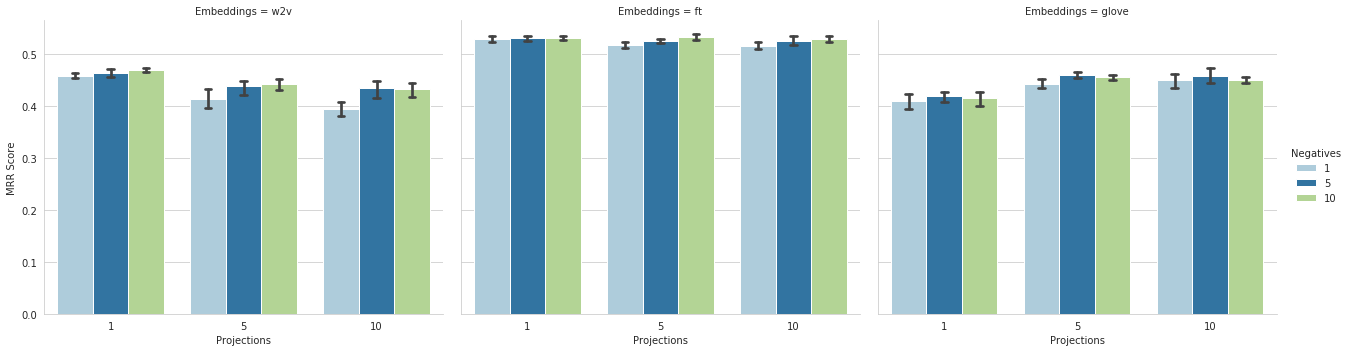
\includegraphics[width=1.\linewidth]{images/CRIM_MRR_score_projection_and_negative_sample.png}
  \caption{CRIM \ac{MRR} score variations by embeddings, projections, and negative sample count.}
  \label{fig:crim_hyper_mrr}
\end{figure}
\begin{figure}[ht!] 
  \centering
  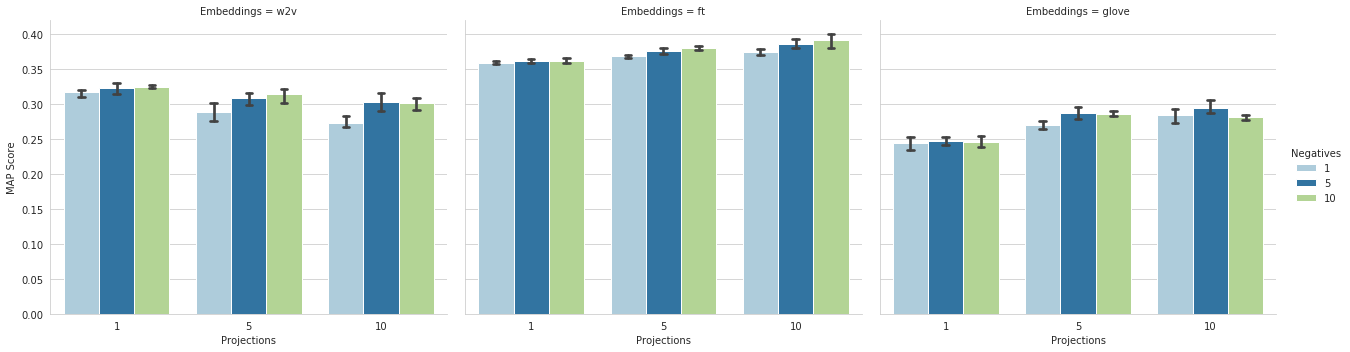
\includegraphics[width=1.\linewidth]{images/CRIM_MAP_score_projection_and_negative_sample.png}
  \caption{CRIM \ac{MAP} score variations by embeddings, projections, and negative sample count.}
  \label{fig:crim_hyper_map}
\end{figure}
Figures~\ref{fig:crim_hyper_mrr},\ref{fig:crim_hyper_map} illustrate plots of our 5-fold cross-validated \ac{MRR} and \ac{MAP} results respectively, generated by non-regularised models configured with different hyperparameter combinations, each trained on three distinct embeddings features.  Standard error bars were added to each plot.  

Increasing the number of projections did not have the same effect across all embeddings spaces.  Word2vec \ac{MRR} and \ac{MAP} results were adversely impacted, especially when a larger projection count was combined with a single negative sample count.  In this case, we measured an MRR and MAP decrease of 14\% and 13.7\% respectively on the 10-projection, single negative sample model, compared to single projection, single negative sample model.  GloVe-trained models were affected by multiple projections; all configurations yielded higher means for both \ac{MRR} and \ac{MAP} readings.  fastText \ac{MRR} is slightly negatively correlated to the number of projections learned but mean \ac{MAP} rose as projections were increased from 1 to 5, and 1 to 10 projections respectively.  However, increasing model complexity by learning 10 projections instead of 5, left only a modest mark on the scores.  In \cref{Eval_CRIM_ProjEmb} we will discover whether these improvements are statistically backed by an \ac{ANOVA} study.

We observed a generally positive effect when augmenting the number of negative samples from a single one to at least five.  In approximately one third of the configurations, we observed an increase of means when  comparing both \ac{MRR} and \ac{MAP} metrics.  The configuration which mostly exploited a negative sample increase was the word2vec, 10-projection model where \ac{MRR} and \ac{MAP} improved by 10.2\% and 11.1\% respectively when 5 negative samples were fed to the model during training, compared to a single negative sample.  Similar to the projections hyperparameter, the improvement garnered when going from 5 to 10 negative samples is subtler, and this holds across all configurations.  

\subsection{Yamane Results}
\begin{table*}\centering
    \begin{tabular}{@{}lcccrr@{}} \toprule
    & \textbf{Clusters} & $\bm{\lambda}$ & \textbf{Neg. Count} & \textbf{Mean MRR} & \textbf{Mean MAP}\\
    \cmidrule{2-6}
    \textit{w2v} & 4 & 0.16 & 5 & 0.538 $\pm$0.017 & 0.390 $\pm$0.029\\
    \textit{GloVe} & 4 & 0.16 & 5 & 0.451 $\pm$0.017 & 0.297 $\pm$0.024\\
    \textit{fastText} & 5 & 0.18 & 5 & 0.533 $\pm$0.014 & 0.396 $\pm$0.016\\
    \bottomrule
    \end{tabular}
    \caption{Yamane hyperparameter settings and 5-fold cross-validated scores.}\label{tab:yamane_settings_scores}
\end{table*}
The results obtained by our implementation of Yamane can be seen in Table~\ref{tab:yamane_settings_scores}.  The outcome more or less adhered to CRIM's where models trained on fastText features outperformed the other two.  GloVe-trained models scored the lowest \ac{MRR} and \ac{MAP}.  In general Yamane edges past CRIM in terms of \ac{MAP} and \ac{MRR} with the only exception being the GloVe model.

Contrary to the other algorithms, Yamane narrowed the gap between word2vec and fastText-trained models.  The edge that fastText features had over word2vec in the \ac{MSE} almost completely disappeared.  As we saw in Figures~\ref{fig:crim_hyper_mrr},\ref{fig:crim_hyper_map}, multiple projections damaged CRIM's performance.  This is contrasted in Yamane, where learning four projection matrices (one per cluster) improved word2vec-trained model's \ac{MRR} and \ac{MAP}.  However, despite this performance boost, we found Yamane models hard to train.  Metrics collected on the validation fold at the end of every epoch, show models that have a tendency to be erratic and which converge surprisingly quickly.  
\begin{figure}[ht!] 
  \centering
  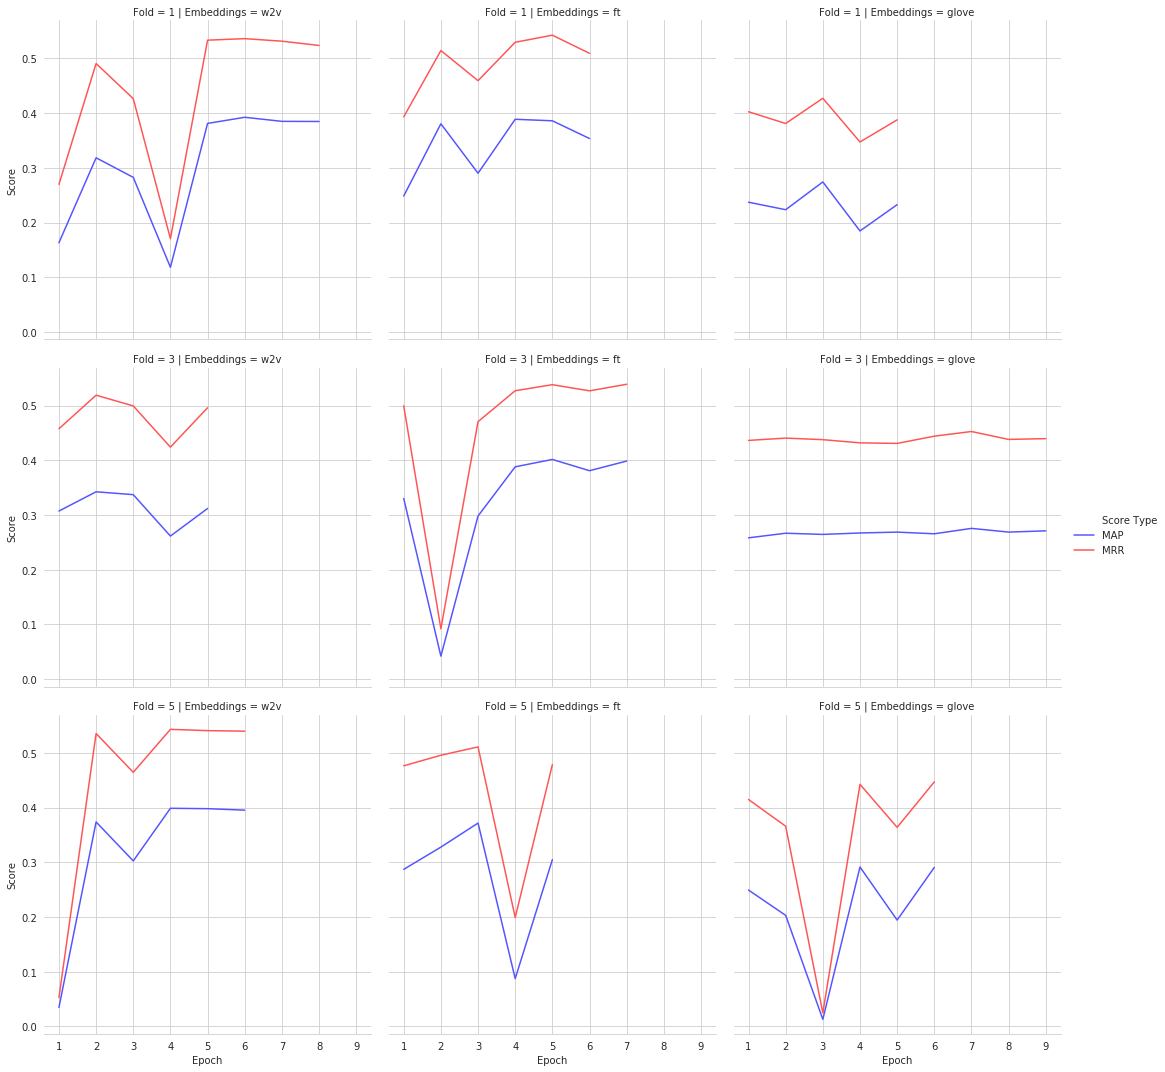
\includegraphics[width=.75\linewidth]{images/Yamane_training_patterns.png}
  \caption{Yamane training patterns on selected folds.}
  \label{fig:yamane_training_patterns}
\end{figure}
We captured training patterns in a matrix displayed in Figure~\ref{fig:yamane_training_patterns}. The rows show the pattern on the arbitrarily chosen 1st, 3rd and 5th data folds, while columns illustrate how the model reacts to the various feature embeddings during the first 10 epochs.  We measured validation \ac{MAP} and \ac{MRR}.  Although the validation fold query terms are always entirely segregated from the training terms, the validations results are sometimes as good as the final results obtained after training an \ac{MSE} model for 700 epochs.  This is especially evident with the  fastText-trained models (middle column).  Large dips often follow the creation of new clusters since the most recent cluster would also be the relatively less trained.  Many more gradient updates are performed in an epoch in Yamane than in CRIM since the model is training on a single positive sample at a time (augmented by 5 negative hypernym candidates randomly drawn during training) and there is no indication in \citet{yamane2016distributional} that the learning rate should be reduced to factor for the smaller batch size.  The absence of patterns both row-wise and column-wise in the plot suggests some form of bias towards the inherent randomness when choosing the training samples, one at a time, with which to train the ensemble's clusters.  Early stopping is evident in all sub-plots with all but one of the examples terminating before the tenth epoch.  Our conservative \textit{patience} setting coupled with the ensemble's propensity to maximise validation performance earlier in the training loop contributed to this phenomenon.

\subsection{Best Models}
\begin{figure}[ht!] 
  \centering
  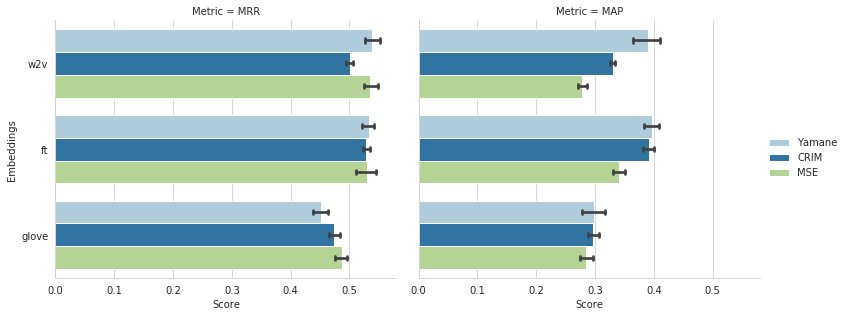
\includegraphics[width=1.\linewidth]{images/Comparison_of_best_performing_algorithms.png}
  \caption{\ac{MRR}, \ac{MAP} scores of best-performing models in projection learning family.}
  \label{fig:part1_best_models}
\end{figure}

\begin{table*}\centering
    \begin{tabular}{@{}clccc@{}} \toprule
    \textbf{Model} & \textbf{Embeddings} & \shortstack{\textbf{Projections/}\\\textbf{Clusters}} & $\bm{\lambda}$ & \textbf{Neg. Count} \\ \midrule
    \multirow{3}{*}{CRIM} & \textit{word2vec} & 1 & 0.10 & 10 \\
    & \textit{GloVe} & 5 & 1.00 & 5\\
    & \textit{fastText} & 10 & 0.00 & 10\\ \cmidrule{2-5}
    \multirow{3}{*}{Yamane} & \textit{word2vec} & 4 & 0.16 & 5 \\
    & \textit{GloVe} & 4 & 0.16 & 5\\
    & \textit{fastText} & 5 & 0.18 & 5\\ \midrule
    & \textbf{Embeddings} & \textbf{Clusters} & \multicolumn{2}{c}{\textbf{Regularised Model}}\\ \cmidrule{2-5}
    \multirow{3}{*}{MSE} & \textit{word2vec} & 25 & \multicolumn{2}{c}{Neighbour} \\
    & \textit{GloVe} & 1 & \multicolumn{2}{c}{Neighbour} \\
    & \textit{fastText} & 1 & \multicolumn{2}{c}{Asymmetric} \\
    \bottomrule
    \end{tabular}
    \caption{Best-performing models' hyperparameter settings.}\label{tab:all_model_best_hyper}
\end{table*}

We conclude this section, by selecting the best-performing configuration of each respective model: \ac{MSE}, CRIM and Yamane.  We ranked every model based on the harmonic mean of the cross-validated \ac{MRR} and \ac{MAP} scores.  The hyperparameter combinations that led to the best models, based on our definition are shown in Table~\ref{tab:all_model_best_hyper} and the scores - together with standard error bars - can be seen in Figure~\ref{fig:part1_best_models}.  The binary cross-entropy models which estimate the similarity between the projected and actual hypernym using the dot-product operation and which allow the presentation of explicit negative examples, seem to generate more accurate hypernyms.  The best \ac{MSE} model scored a mean 0.341 \ac{MAP} when trained on fastText embeddings.  This score was only bettered by the binary cross-entropy models trained on fastText, with a margin of 16.24\% and 14.84\% with Yamane and CRIM respectively.  The Yamane model scored a mean 0.3901 \ac{MAP} on the word2vec trained model, the only tested model to bridge the word2vec/fastText divide on \ac{MAP}.  By way of contrast, the next best \ac{MAP} score we recorded was 0.3302 (CRIM) while from the \ac{MSE} models, the highest score obtained was 0.278.  The GloVe embeddings seemed to be the least affected by different models: the highest (Yamane) and lowest (MSE) scores different by only 1.2 points.

\ac{MSE} models are more competitive with respect to \ac{MRR} indicating that either model type is more or less equally capable of generating a correct highest ranked hypernym.  Yamane and MSE scored 0.539 and 0.536 respectively - practically equivalent results - on the word2vec trained models, while CRIM trailed behind with 0.502.  fastText features dampened the effect of the model, with cross-validated scores of 0.533, 0.528 and 0.529 obtained on Yamane, CRIM and MSE models respectively.  Finally, the MSE model coaxed the top \ac{MRR} score of 0.487 from among GloVe-trained models.  However, this score trails 1.46 points behind the worst-performing model in the rest of the cohort (CRIM trained on word2vec).

Our experiments did not exhaust all reasonable model configurations, so these results are not necessarily conclusive.  We will determine if the differences in our collected data are statistically significant in \cref{Eval_BestOutOf3}, where we evaluate our findings according to the \ac{ANOVA} framework.  In the next section we shift focus to the SemEval-2018 Task 9 English, general-purpose task and the application of the knowledge gathered from these experiments to a "real life" problem setting.

\section{Experiments on Shared Task Corpus and Data}
Based on its performance, quick convergence and configurability, we applied our CRIM implementation on the Shared Task.  Our implementation is distinguished from the original technical setup \citep{bernier2018crim}, by learning the projection matrices and tuning the embeddings in two separate training phases, enabling us to accelerate convergence.  Beside word2vec word embeddings, we additionally fit our model on GloVe and fastText features.

We focused on the English, general-purpose task which was accompanied by the largest corpus and dataset.  In a novel departure from the Combined Dataset, and other dataset used in the experiments we reviewed, the Shared Task organisers categorised each query term as either \textit{concept} or \textit{entity}.  The objectives of our experiments were to:
\begin{itemize}
    \item With frozen embeddings
    \begin{enumerate}
        \item At the most basic level, find out if our implementation matches the published performance of CRIM;
        \item Determine whether the combination of projection layers and embeddings has some effect on the validation score on the test set;
        \item Train the model on concept, entities separately and combined, and each time validate it on only concepts, only entities, and both term types together.  In this way we will investigate whether entity (or concept) hypernymy encodes its own signal which cannot be generalised unless the model is first exposed to actual entity (or concept) examples;
        \item Experiment with an \ac{MTL} setup whereby we train a common feature extractor connected to two logistic regression classifier heads, which learn optimal coefficients for concepts and entities separately;
    \end{enumerate}
    \item Towards tuned embeddings
    \begin{enumerate}
        \item For each embeddings space, find the best model in terms of the harmonic mean of \ac{MAP} and \ac{MRR}, and apply a simple transfer learning method to tune embeddings whilst keeping the previously trained projection matrices static;
    \end{enumerate}
\end{itemize}

\subsection{Effect of Projection Layers and Embeddings on Model}
\begin{figure}[ht!] 
  \centering
  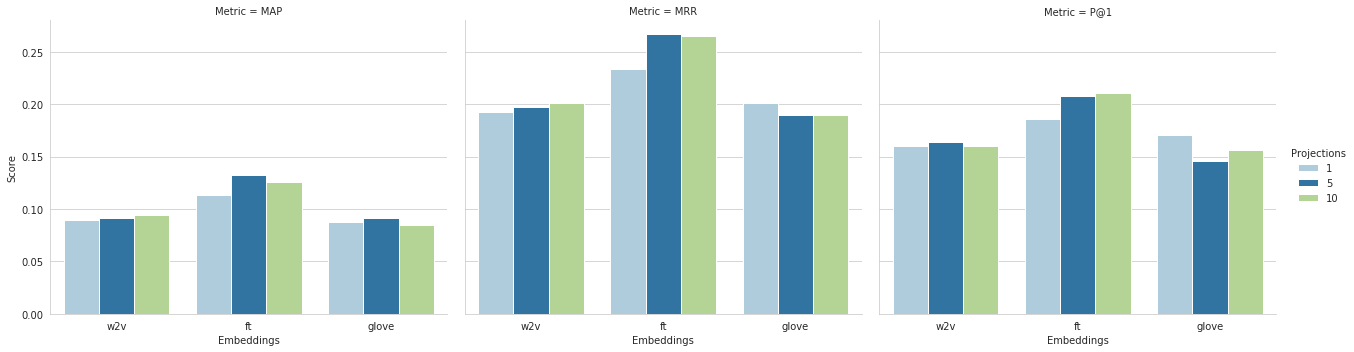
\includegraphics[width=1.\linewidth]{images/semeval_crim_proj_embed.png}
  \caption{\ac{MRR}, \ac{MAP} and P$@1$ scores of CRIM, by embeddings spaces and projection layer count.}
  \label{fig:semeval_crim_proj_embed}
\end{figure}
We present the \ac{MAP}, \ac{MRR} and P$@1$ results of models trained and validated on a combination of concepts and entities in Figure~\ref{fig:semeval_crim_proj_embed}.  fastText embeddings trained on 5  projection layers returned the best \ac{MAP} and \ac{MRR} scores, at 0.133 and 0.267 respectively.  The fastText, 10 projection layer model obtained the highest P$@1$ score at 0.211, a subtle improvement on the 0.208 result recorded by the 5 projection layer model.

Unlike the experiments on the Combined Dataset, increasing projections had a positive, albeit slight, effect on the word2vec-trained models.  In fact, the best word2vec results were observed with the 10 projection layer model.  GloVe delivered results comparable to word2vec, although increasing the projections had an overall negative effect on all scores except \ac{MAP}.

\subsection{Segregation of Training Data by Query Type}
We discovered that performance is influenced by the words with which we choose to fit a model.  From what we could empirically observe, the best strategy was to train a model with a mix of entities and concepts.  Training a model on concepts or entities exclusively invariably damaged its ability to generate hypernyms for the \textit{type} of query terms it has not observed during training.  For every embeddings space, we first selected the best performing model in terms of projection count when trained and validated on concepts and entities.  Then, we trained each model on the word types separately, and evaluated it on all word type combinations.  The cross-tabulated scores can be seen in Table~\ref{tab:semeval_wordtype_results}.
\begin{table*}\centering
\begin{tabular}{@{}llrrcrrcrr@{}}\toprule
& & \multicolumn{8}{c}{\textbf{Tested On}}\\ 
\cmidrule{3-10}
\multicolumn{2}{c}{\multirow[c]{2}{*}{\textbf{Trained On}}} & \multicolumn{2}{c}{Concept} & \phantom{a} & \multicolumn{2}{c}{Entity} & \phantom{a} & \multicolumn{2}{c}{Both}\\ 
\multicolumn{2}{c}{} & \textit{MRR} & \textit{MAP} && \textit{MRR} & \textit{MAP} && \textit{MRR} & \textit{MAP}\\
\cmidrule{3-4} \cmidrule{6-7} \cmidrule{9-10}  
\multirow{3}{*}{\textit{word2vec}} 
& Concept & 0.109 & 0.050 && 0.070 & 0.029 && 0.098 & 0.044\\
& Entity & 0.029 & 0.015 && 0.300 & 0.139 && 0.109 & 0.051\\
& Both & 0.160 & 0.073 && 0.299 & 0.143 && 0.201 & 0.094 \\ \midrule

\multirow{3}{*}{\textit{fastText}} 
& Concept & 0.208 & 0.099 && 0.305 & 0.132 && 0.237 & 0.109\\
& Entity & 0.055 & 0.026 && 0.394 & 0.195 && 0.155 & 0.076\\
& Both & \textbf{0.211} & \textbf{0.105} && 0.398 & 0.199 && \textbf{0.267} & \textbf{0.133}\\ \midrule

\multirow{3}{*}{\textit{GloVe}} 
& Concept & 0.106 & 0.045 && 0.036 & 0.014 && 0.086 & 0.036 \\
& Entity & 0.033 & 0.013 && \textbf{0.445} & \textbf{0.206} && 0.155 & 0.070 \\
& Both & 0.119 & 0.059 && 0.359 & 0.170 && 0.190 & 0.092\\ 
\bottomrule
\end{tabular}
\caption{Test results for models trained on concepts, entities, concepts and entities.}\label{tab:semeval_wordtype_results}
\end{table*}

\begin{table*}\centering
\begin{tabular}{@{}llrrcrrcrr@{}}\toprule
& & \multicolumn{8}{c}{\textbf{Tested On}}\\ 
\cmidrule{3-10}
\multicolumn{2}{c}{\multirow[c]{2}{*}{\textbf{Trained On}}} & \multicolumn{2}{c}{Concept} & \phantom{a} & \multicolumn{2}{c}{Entity} & \phantom{a} & \multicolumn{2}{c}{Both}\\ 
\multicolumn{2}{c}{} & \textit{MRR} & \textit{MAP} && \textit{MRR} & \textit{MAP} && \textit{MRR} & \textit{MAP}\\
\cmidrule{3-4} \cmidrule{6-7} \cmidrule{9-10}  
\textit{word2vec} & Both & 0.161 & 0.074 && \textbf{0.339} & \textbf{0.164} && 0.214 & 0.100 \\ 
\textit{fastText} & Both & 0.194 & 0.094 && 0.403 & 0.200 && 0.256 & 0.125\\ 
\textit{GloVe} & Both & 0.125 & 0.059 && \textbf{0.402} & \textbf{0.193} && 0.207 & 0.099\\ 
\bottomrule
\end{tabular}
\caption{Test results for best \ac{MTL} models.}\label{tab:semeval_mtl}
\end{table*}

In general, the best performance is coaxed out a model when it is trained on a mix of concept and entities.  However, the fastText model trained on concepts exclusively is an exception: it still managed a comparatively decent 0.305 \ac{MRR} and 0.132 \ac{MAP}.  The reverse effect was not observed: training fastText on only entities, impaired the model's ability to generate hypernyms for concept terms.  We also noted that models trained and evaluated on entities yielded the best scores.  This is possibly due to the distribution of hypernyms within the entity category as observed in Figure~\ref{fig:shared_task_mfh}, where around 8\% of all entity tuples are instances of \textit{person}, \textit{city} or \textit{writer}.  GloVe embeddings were particularly adept at generating hypernyms for entity words, given that the model was trained exclusively on entities.  The GloVe Entity-Entity model scored the highest \ac{MRR} and \ac{MAP}.

\subsection{Multi-task Learning Setup}
Considering the additional complexity that went into the model's structure, training and prediction algorithms, the \ac{MTL} setup delivered modest gains.  Specifically, we observed development in the ability of word2vec and GloVe models to generate hypernyms for entity queries when trained on concepts and entities.  word2vec \ac{MRR} and \ac{MAP} were 13.4\%  and 14.6\% higher than the single classifier scores respectively.  GloVe \ac{MRR} and \ac{MAP} were 12\% and 13.5\% than the single classifier scores respectively.  In all cases, the best results were observed from models initialised with 5 projection layers, irrespective of the word embeddings space.  \ac{MRR} and \ac{MAP} results obtained from the \ac{MTL} models can be viewed in Table~\ref{tab:semeval_mtl}.

\subsection{Transfer Learning Setup}
\begin{figure}[!ht]
    \centering
    \subbottom[MRR]{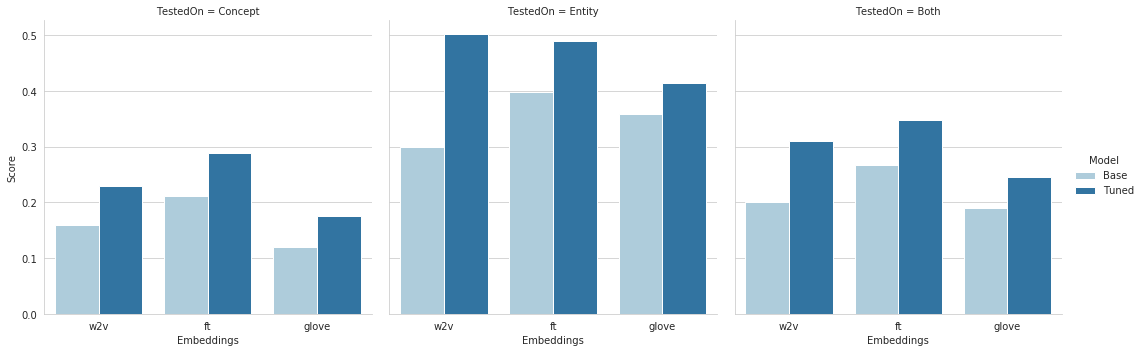
\includegraphics[width=0.8\textwidth]{images/semeval_mrr_tuned.png} }\qquad
    \subbottom[MAP]{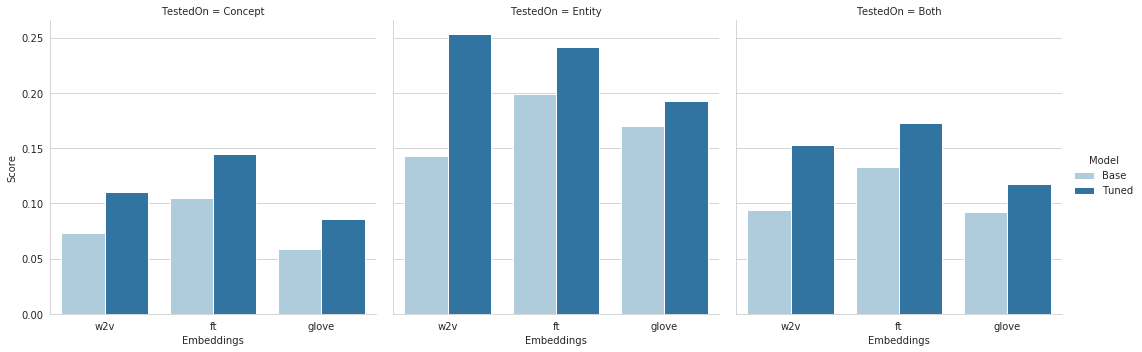
\includegraphics[width=0.8\textwidth]{images/semeval_map_tuned.png}}%
    \caption{Boost on \ac{MRR} and \ac{MAP} due to embeddings tuning.}        
    \label{fig:embeddings_boost}
\end{figure}
Our transfer learning mechanism successfully boosted models' performance in all embeddings scenarios.  Figure~\ref{fig:embeddings_boost} displays the \ac{MRR} (top) and \ac{MAP} (bottom) scored by the base model, trained on frozen embeddings (light shading), and tuned model (dark shading) in which we trained the embeddings but froze the projections.  The plot shows the returned scores when the models were tested on concepts (left), entities (centre) and concept+entity (right).

The models perform better on generating hypernyms for entities than for concepts, irrespective of the embeddings used.  fastText retains its edge even after embeddings tuning.  Entities are the only exception: a tuned word2vec model scored 0.501 \ac{MRR} and 0.253 \ac{MAP}, slightly better than fastText at 0.490 and 0.242 respectively.  word2vec benefited the most from the embeddings tuning: \ac{MRR} and \ac{MAP} increased by 53.79\% and 62.31\% in the concept+entity evaluation. 

From all the experiments we executed on Shared Task dataset, our tuned fastText embeddings yielded the highest MRR/MAP scores on the concept+entity test dataset.  The model returned a respectable \textbf{0.348}/\textbf{0.173} which would have placed it third overall in the Shared Task submission leader-board.